\chapter{Russian Post in Mongolia}  


\begin{figure}[htbp]
\centering
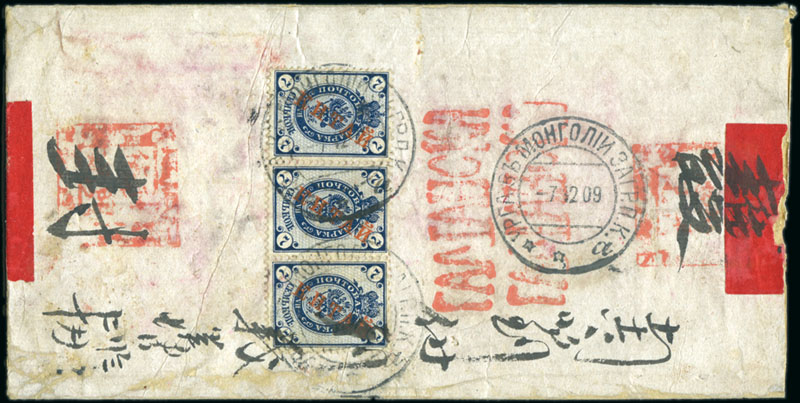
\includegraphics[width=.95\textwidth]{../russian-post-in-mongolia/10123.jpg}
\caption{ 
10123 URGA: 1879 Native cover from Urga to Peking, dated "14th Day, 8th Moon, 1879", 
franked with Russia Arms 3k and 5k cancelled by brush strokes 
(the first type of cancel used in Mongolian offices) paying the
8k rate, some minor peripheral faults, rare, only about 12 covers known
from Urga with pen / brush stroke cancel (brush strokes are much rarer)
Note: Recorded in the BJRP no.36 (1965) p.26
Provenance: Ex Adgey-Edgar
\euro 8,000.00 
} 
\end{figure} 

\begin{figure}[htbp]
\centering
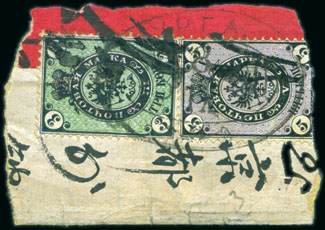
\includegraphics[width=.50\textwidth]{../russian-post-in-mongolia/10124.jpg}
\caption{ 
10124 URGA: Fragment with 3k and 5k tied by a fairly good strike of the 
rare Urga 8.IX.1880 Type 3A oval ds (rated RR by Hellrigl), 
5k trimmed at foot, very few examples of this cancellation are known.
Provenance: Ex Tolman
\euro 400.00
} 
\end{figure}    

\begin{figure}[htbp]
\centering
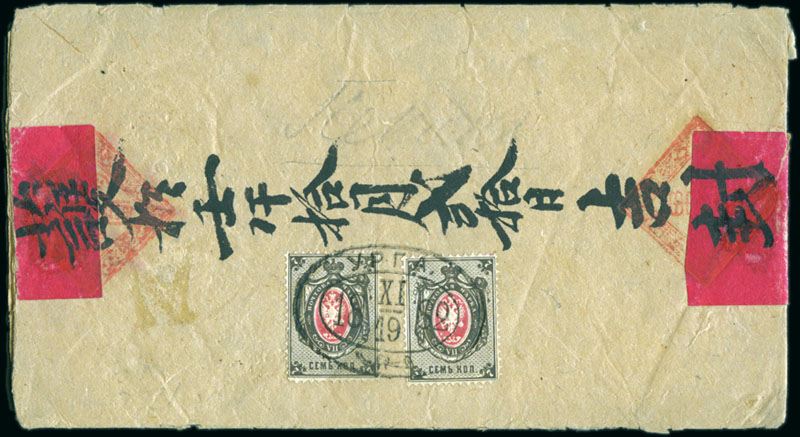
\includegraphics[width=.95\textwidth]{../russian-post-in-mongolia/10125.jpg}
\caption{ 
10125 URGA: 1882 Native cover to Peking with two 7k tied by a very good 
strike of the Urga 19.XI.1882 type 3B oval ds, paying double the internal 
rate, scarce.
Note: Illustrated in "Stamps of the Russian Empire Used Abroad" pg.314 by 
Tchilinghirian \& Stephen
\euro 2,000.00 
} 
\end{figure} 

\begin{figure}[htbp]
\centering
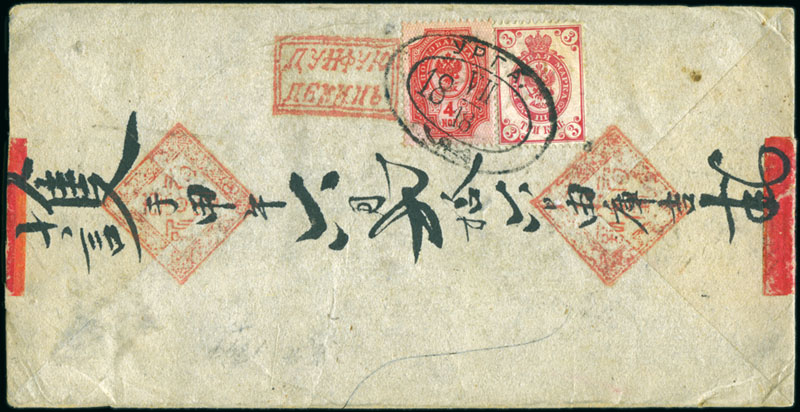
\includegraphics[width=.95\textwidth]{../russian-post-in-mongolia/10126.jpg}
\caption{ 
10126 URGA: Native cover sent from Urga to Peking with Russia 3k and 4k paying 
the single internal rate, tied by a single fine strike of the Urga 18.VII 
type 3c oval ds, fine and neat franking, showing attractive "DUN-FU-YU" 
boxed cachet in red

Provenance: Ex Tolman
\euro 400.00 
} 
\end{figure}    

\begin{figure}[htbp]
\centering
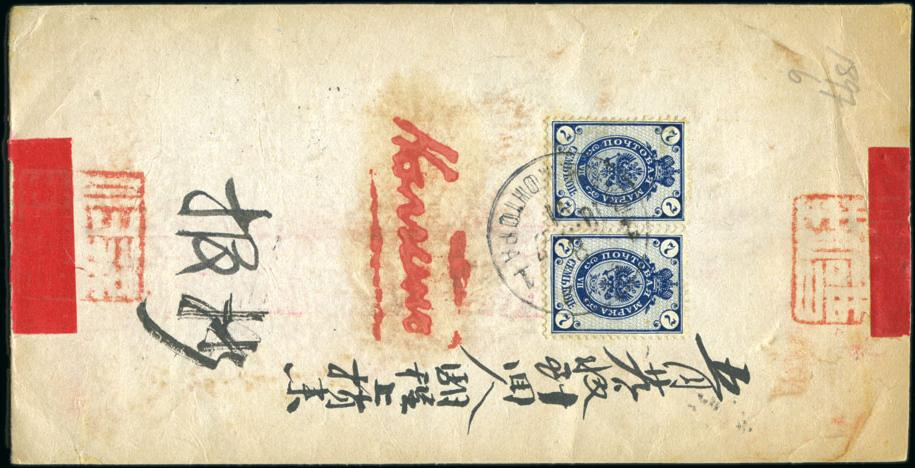
\includegraphics[width=.95\textwidth]{../russian-post-in-mongolia/10127.jpg}
\caption{ 
10127 URGA: 1897 Native cover to Kalgan, franked with two Russia 
Arms 7k blue paying double rate, tied by a single Urga 8.VI.97 type 4 
large numerals cds in black, fine
Provenance: Ex Tolman
\euro 300.00.
} 
\end{figure}    



    